

%==============================================
\subsection{Godunov's Method}\label{chap:godunov}
%==============================================










%============================================
\subsubsection{Method}
%============================================

Godunov's method arises from the integral form of the conservation law so that discontinuous solutions are allowable.

For the one dimensional method, we discretize the spatial domain into $M$ computing cells of regular size, and assume that the initially continuous data is represented by piecewise constant distribution of data, see fig. \ref{fig:piecewise-constant}.



\begin{figure}[H]
	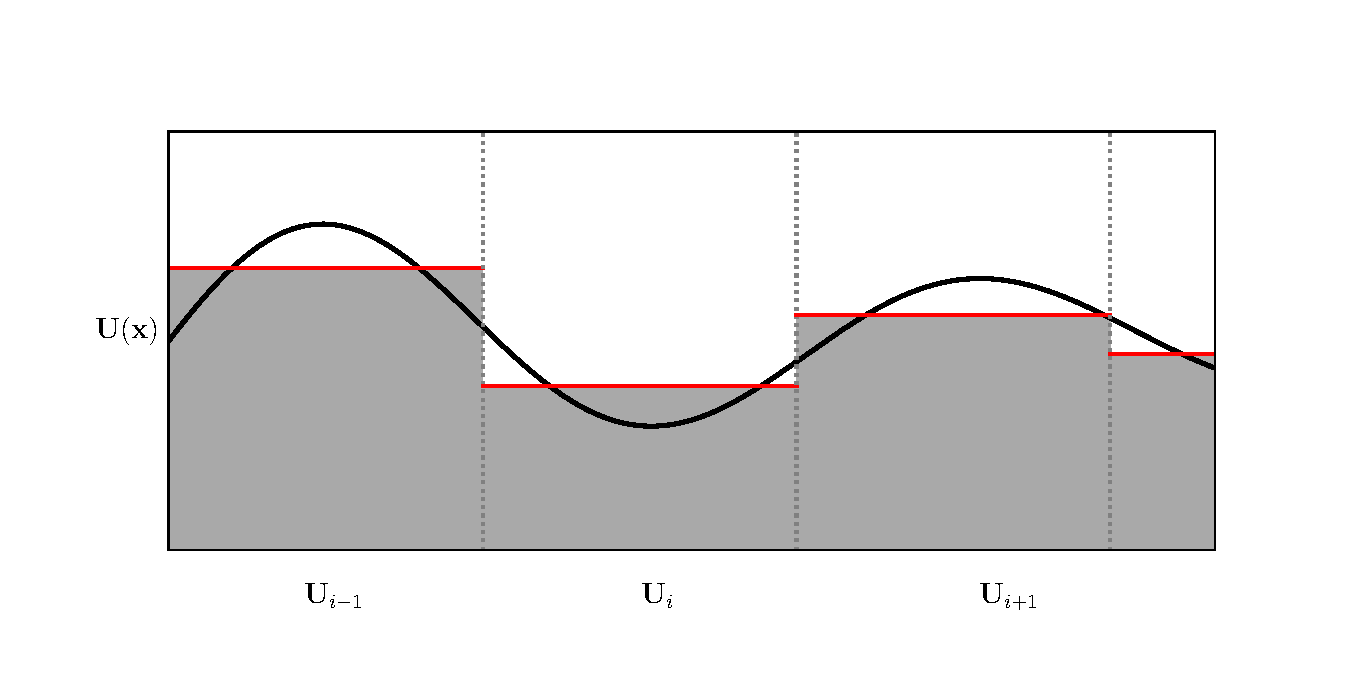
\includegraphics[width=\textwidth]{./figures/piecewise_const.pdf}%
	\caption{	
		A piecewise constant representation of continuous data among cells.
		\label{fig:piecewise-constant}
		}
\end{figure}

Having a collection of piecewise constant states, we effectively have to solve local Riemann problems with data $\U_i$ as $\U_L$ and $\U_{i+1}$ as $\U_R$, centered at the intercell boundary positions $x_{i+\half}$.
The solution of the Riemann problem will depend on $\frac{\bar{x}}{\bar{t}}$, where $\bar{x}$ and $\bar{t}$ are in local coordinates to the specific Riemann problem under consideration. 
$\bar{x}$ is zero at $x_{i+\half}$ and increasingly negative with decreasing $i$.
$\bar{t}$ is zero at the current timestep.


Now suppose that we have solved the Riemann problem at the position $x_{i+\half}$ with left state $\U_L = \U_i$ and right state $\U_R = \U_{i+1}$.
Then, as time evolves, how will the state at $x_{i+\half}$ change?

Recall that the elementary waves travel along characteristics, and that the characteristics are straight lines on the $x-t$ - diagram (see fig. \ref{fig:riemann-solution}.
Then the state at $x_{i+\half}$, which is where the dividing line between the two initial states is, will be given by the solution of the Riemann problem at the position $\bar{x} = 0$, and will remain the same for all $\bar{t} > 0$.
(This is assuming there is nothing else that might disturb the current situation.)


Using that fact, it can be derived that (see \cite{toro}) 

\begin{align}
	\U^{n+1}_i = \U^n_i + \frac{\Delta t}{\Delta x} \left[\F(\U_{i-\half}) - \F(\U_{i+\half}) \right] \label{eq:godunov-discretized}
\end{align}

where $\U_{i-\half}$ and $\U_{i+\half}$ are the solutions to the Riemann problems at $x_{i-\half}$ and $x_{i+\half}$, respectively.


It is noteworthy that this is an exact solution to a piecewise constant initial state.




Lastly, we need to limit the time step size.
We mustn't allow for a wave to be able to travel further than one cell length between two timesteps, otherwise we get bogus results.
Remember that we assumed that the state at $x_{i+\half}$ doesn't change after $\bar{t} > 0$.
This is only satisfied if the wave doesn't reach the boundary of the neighbouring cell.

This time step restriction is imposed by the CFL condition:

\begin{align}
	\Delta t_{max} \leq \frac{C_{cfl} \Delta x}{|S_{max}^n|} \label{eq:godunov-cfl}
\end{align}


where $S_{max}^n$ is the highest wave propagation speed at the current time, and $C_{cfl} \in [0, 1($ is the Courant number.


However, this is not the most practical way of doing things.
In 2D, using dimensional splitting, we'd have to first solve everything in one direction to find the wave speeds, then advance the time step of the sweep, then do the other sweep and hope that the maximal wave velocity won't be greater than the one of the previous sweep.
Or re-do the first sweep iteratively until we get decent time steps.

Instead, we use the estimate

\begin{align}
	S^n_{max} = \max\{ |u_i^n| + a_i^n \}
\end{align}

This is not always accurate, and the wave speed can be underestimated, leading to instabilities.
To combat this, we just need to choose a lower $C_{cfl}$.
Toro recommends to use $C_{cfl} < 0.8 - 0.9$.













%===================================================================
\subsubsection{Implementation Details}\label{chap:godunov-details}
%===================================================================


The cells are stored as an array of \verb|struct cell| that stores both primitive states, \texttt{prim}, as  \texttt{struct pstate}, and conserved states, \texttt{cons}, as \texttt{struct cstate}.
Furthermore they have \texttt{struct pstate pflux} and \texttt{struct cstate cflux} to store fluxes of primitive and conserved variables.


The grid is set up as follows:
In 1D, it is a 1D array of \texttt{struct cell}.
In 2D, it is a 2D array.
Indices (0, 0) represent the lower left corner of the simulation domain.
First index is in x direction, i.e. (nx - 1, 0) is at the coordinates (x = xmax, y = 0).


The flux at $x_{i+\half, j}$ and $y_{i, j+\half}$ are stored in \texttt{cflux} or \texttt{pflux} of cell \verb|grid[i, j]|, depending whether you're storing primitive or conserved variables.
For the Godunov scheme, we need conserved variables.
For advection, we only deal with primitive variables.
Because we're doing dimensional splitting, it suffices to have only one storage place, as they will be used in successive order.
See section \ref{chap:dimensional-splitting} for details.

We can afford to store $x_{i+\half}$ at cell $i$ because we have at least 1 extra virtual boundary cell which is used to apply boundary conditions, so the flux at $x_{-\half}$ will be stored in \verb|grid[BC-1]|, where \texttt{BC} is the number of boundary cells used, defined in \texttt{defines.h}.
 

If the grid is only in 1D, then all the above definitions still apply as if y didn't exist.



The related functions are written in \texttt{/program/src/solver/godunov.c} and \texttt{/program/src/solver/godunov.h}.
The hydro related functions are called in the main loop in \texttt{/program/src/main.c} when \verb|solver_step(...)| is called.

The \verb|solver_step(...)| function does the following for the 1D case:
\begin{itemize}
	\item 	Reset the stored fluxes from the previous timestep to zero
	\item 	Compute the primitive states for all cells from the updated conserved states
	\item 	Impose boundary conditions (section \ref{chap:boundary-conditions})
	\item 	Find the maximal timestep that you can do by applying the CFL condition \ref{eq:godunov-cfl}.
	\item 	Compute fluxes:
	\begin{itemize}
		\item 	For every cell pair $(i, i+1)$, solve the Riemann problem (see section \ref{chap:riemann}) to find the flux $\F_{i+\half}$.
		\item 	Store the flux $\F_{i+\half}$ in the \texttt{struct pstate pflux} struct of the cell $i$.
				\texttt{struct pstate} is a struct that contains the primitive state, i.e. density $\rho$, velocity $u_x$, $u_y$, and pressure $p$.
	\end{itemize}
	\item 	Update the states: Effectively compute $\U^{n+1}$ at this point using $\U_i^n$, the flux $\F_{i+\half}$ stored in every cell $i$, and the flux $\F_{i-\half}$ stored in every cell $i-1$ following eq. \ref{eq:godunov-discretized}.
\end{itemize}





